%%%%%%%%%%%%%%%%%%%%%%%%%%%%%%%%%%%%%%%%%%%%%%%%%%%%%%%%%%%%%%%%%%%%%%%%%%%%%%%%%%%%
% Do not alter this block (unless you're familiar with LaTeX
\documentclass{article}
\usepackage[margin=1in]{geometry} 
\usepackage{amsmath,amsthm,amssymb,amsfonts, fancyhdr, color, comment, graphicx, environ}
\usepackage{xcolor}
\usepackage{mdframed}
\usepackage[shortlabels]{enumitem}
\usepackage{indentfirst}
\usepackage{hyperref}
\usepackage{algorithm}% http://ctan.org/pkg/algorithm
\usepackage[noend]{algpseudocode}% http://ctan.org/pkg/algorithmicx
\usepackage{graphicx}
\hypersetup{
    colorlinks=true,
    linkcolor=blue,
    filecolor=magenta,      
    urlcolor=blue,
}


\pagestyle{fancy}


\newenvironment{problem}[2][Problem]
    { \begin{mdframed}[backgroundcolor=gray!20] \textbf{#1 #2} \\}
    {  \end{mdframed}}

% Define solution environment
\newenvironment{solution}
    {\textit{Soln:}}
    {}

\renewcommand{\qed}{\quad\qedsymbol}

% prevent line break in inline mode
\binoppenalty=\maxdimen
\relpenalty=\maxdimen

\graphicspath{ {./images/} }

%%%%%%%%%%%%%%%%%%%%%%%%%%%%%%%%%%%%%%%%%%%%%
%Fill in the appropriate information below
\lhead{Anmol Lingan Gouda Patil}
\rhead{COT5405} 
\chead{\textbf{Homework 1  Due: 11 Oct 2021 11:59pm}}
%%%%%%%%%%%%%%%%%%%%%%%%%%%%%%%%%%%%%%%%%%%%%
\begin{document}
\begin{mdframed}[backgroundcolor=yellow!20]
\textbf{Consider undirected graphs that have n nodes and at most n+8 edges. For these graphs, design an efficient algorithm that finds the minimum spanning tree.} 
\end{mdframed}

\begin{problem}{1}
\textbf{[10 pts]} Design a correct algorithm and show it in pseudo-code.
\end{problem}
\begin{solution}
\begin{algorithm}
\caption{Find minimum spanning tree Depth First Search}\label{dfs}
\begin{algorithmic}[1]
% \KwResult{A boolean as to whether a cycle exists or not}
\Procedure{IsMST}{$G$}
% initialization\;
    \For{\texttt{each vertex $v$ in $G$}}
        \State \texttt{$visited[u] \gets false$}
    \EndFor
    \State \texttt{$maxEdge \gets random edge from$ $G$}
    \For{\texttt{each vertex $v$ in $G$}}
        \If {$v$ is not visited}
            \If {$DFSUtil(G, v, -1, visited, maxEdge) = true$}
                \State \Return \texttt{$true$}
            \EndIf
        \EndIf
    \EndFor
    \State \Return $false$
\EndProcedure
\newline
\Procedure{DFSUtil}{$G,v,parent,visited,maxEdge$}
    \State \texttt{$visited[v] \gets true$}
    \For{\texttt{each neighboring vertex $u$ of $v$}}
        \State \texttt{$maxEdge \gets maximumOf(maxEdge, edge(u ,v))$}
        \If{$u$ is not visited}
            \If {$DFSUtil(G, u, v, visited, maxEdge) = true$}
                \State \Return \texttt{$true$}
            \EndIf
        \Else
            \If {$u \ne parent$} \Comment{A backedge}
                \State \texttt{$G \gets G - maxEdge$}
                \State \Return $true$
            \EndIf
        \EndIf
    \EndFor
    \State \Return $false$
\EndProcedure
\end{algorithmic}
\end{algorithm}
\end{solution}

\begin{problem}{2}
\textbf{[10 pts]} Provide proof of the algorithm's correctness.
\end{problem}
\begin{solution}
The above algorithm's core logic behind finding a minimum spanning tree is by eliminating the maximum edges. In the given case there are 8 more edges than vertices. Which implies if vertices are say $V$ = v then edge count is $E$ = v+8.

The correctness of the algorithm can be proved by the method of proof by contradiction.

\underline{\textit{Note:}} The above algorithm has to be run 9 times in order to remove the maximum weighted edges to get a minimum spanning tree. This is because a tree can only have $V-1$ edges, which implies in the current case that 9 edges from V+8 edges have to be removed in order to obtain a tree.

\begin{proof}:
Assume the above algorithm, after running for stated number of iterations on a graph \textbf{$G$} does not produce a minimum spanning tree. This means that the graph that is obtained at the end of running the algorithm for so many iterations has at least one edge heavier than what an ideal minimum spanning tree would arise out of \textbf{$G$}.
Since the algorithm always eliminates the maximum edge it encounters during a cycle, at every iteration the edge that is maximum so far in the graph is removed. This can be easily proved by understanding that DepthFirstSearch always detects cycle after it has visited every node in a connected component and therefore all edges that are not part of cycle are visited at least once.
Thus after 9 iterations the above algorithm removes the top 9 weighted edges, making the graph a tree with least possible weight, which essentially is a minimum spanning tree.
This contradicts our assumption. Therefore it can be proved that the  algorithm $Find Minimum Spanning Tree Depth First Search$ with given preconditions on $V$ and $E$ always produces a minimum spanning tree after E-V+1 iterations.
\end{proof}
\end{solution}

\begin{problem}{3}
\textbf{[10 pts]} Find and prove the algorithm's running time.
\end{problem}
\begin{solution}
The time complexity of the algorithm above is O(V) where V is the number of nodes.
\begin{itemize}
\item We have a precondition that the maximum number of edges that the graph can have is V + 8.
\item 
A tree contains V-1 edges and a cycle should contain atleast V edges.
\item The above algorithm visits every node once.
\item To find the minimum spanning tree, the above algorithm visits atmost V nodes before discovering a back edge and finally discarding the maximum weight edge.
\item However, since there are 9 more edges than required number of edges that can satisfy the condition of a tree(V-1 edges). This algorithm has to be run for a maximum of 9 times. Resulting in the following time complexity:
$9 \times O(V)$

\item Why order of O(V)? because the algorithm is similar to the first algorithm presented for detecting a cycle.
Therefore a constant times O(V) 
\item $c \times O(V) = O(V)$.
\item If there is no cycle it traverses all nodes only once before terminating, also O(V).
\end{itemize}
\end{solution}


\begin{problem}{4}
\textbf{[20 pts]} Implement the algorithm in a compiled language.
\begin{enumerate}
    \item Write a graph generator.
    \item Write test code to validate that the algorithm finds a spanning tree.
    \item Test the algorithm for increasing graph sizes.
    \item Plot the running time as a function of size to verify that the asymptotic complexity in step 3 matches experiments.
\end{enumerate}
\end{problem}
\begin{solution}
Running time as a function of size to verify the asymptotic complexity.
\begin{figure}[h]
    \centering
    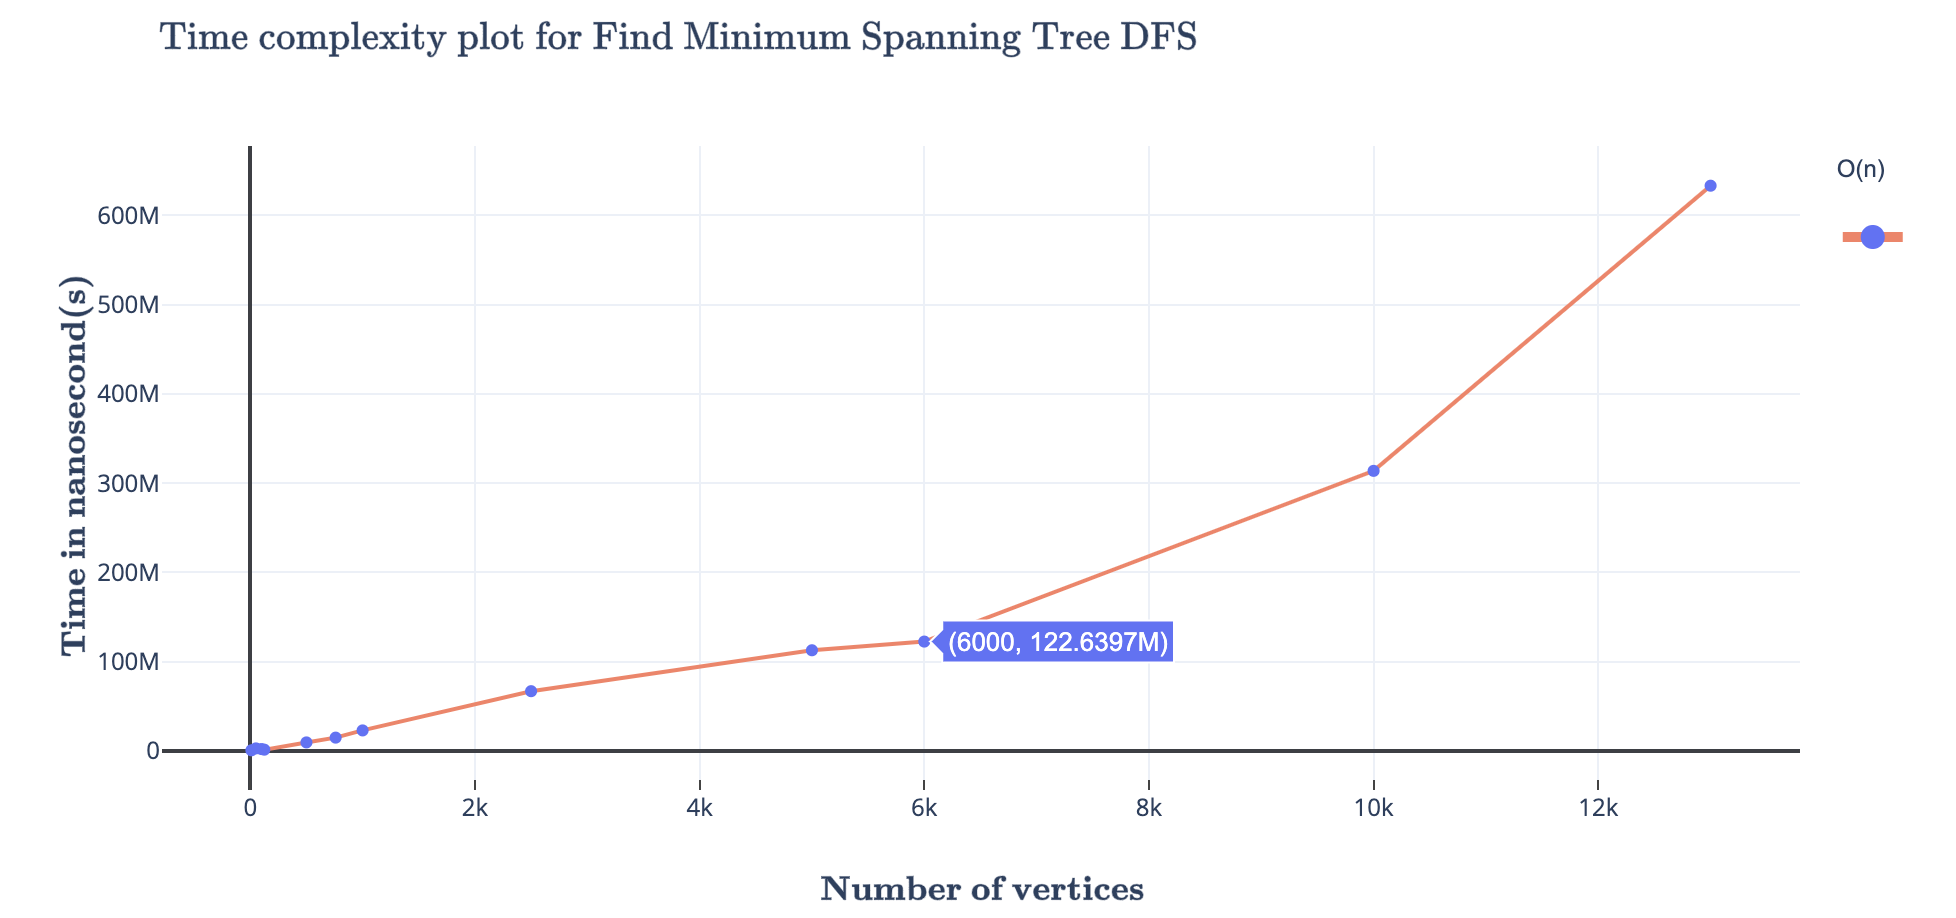
\includegraphics[scale=0.5]{Alg-2}
    \caption{Find Minimum Spanning Tree Depth First Search performance}
    \label{fig:my_label}
\end{figure}
\end{solution}
\end{document}
